\documentclass[tikz,border=5pt]{standalone}
\usepackage{amsmath}
\usetikzlibrary{arrows.meta}

\definecolor{inFill}{HTML}{DCE9F7}
\definecolor{inBorder}{HTML}{2563EB}
\definecolor{tgFill}{HTML}{DCFCE7}
\definecolor{tgBorder}{HTML}{15803D}
\definecolor{blFill}{HTML}{F3F4F6}
\definecolor{blBorder}{HTML}{6B7280}
\definecolor{resFill}{HTML}{FFEDD5}
\definecolor{resBorder}{HTML}{C2410C}
\definecolor{meanFill}{HTML}{FEF3C7}
\definecolor{meanBorder}{HTML}{B45309}
\definecolor{evFill}{HTML}{F3E8FF}
\definecolor{evBorder}{HTML}{7E22CE}
\definecolor{arrGray}{HTML}{374151}

\begin{document}
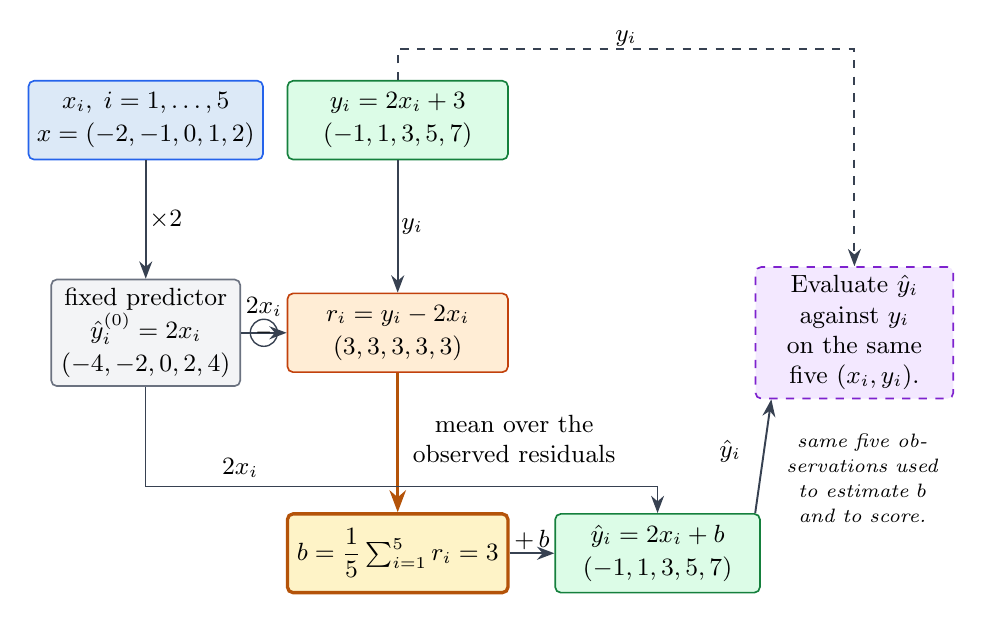
\begin{tikzpicture}[
  x=1cm, y=1cm,
  box/.style={rounded corners=2pt, line width=0.6pt, align=center,
              inner sep=3pt, minimum height=1.0cm, font=\small},
  arr/.style={draw=arrGray, line width=0.7pt, -{Stealth[length=2.2mm]}},
  elbow/.style={draw=arrGray, line width=0.5pt, -{Stealth[length=2.2mm]}},
  amberarr/.style={draw=meanBorder, line width=1.0pt, -{Stealth[length=2.8mm]}},
  lab/.style={font=\small, inner sep=1pt}
]

% ---- Row 1 : data ----------------------------------------------------
\node[box, fill=inFill, draw=inBorder, minimum width=2.6cm] (input) at (1.5,7.0)
  {$x_i,\; i=1,\dots,5$\\[1pt] $x=(-2,-1,0,1,2)$};
\node[box, fill=tgFill, draw=tgBorder, minimum width=2.8cm] (target) at (4.7,7.0)
  {$y_i = 2x_i+3$\\[1pt] $(-1,1,3,5,7)$};

% ---- Row 2 : computation ---------------------------------------------
\node[box, fill=blFill, draw=blBorder, minimum width=2.4cm] (baseline) at (1.5,4.3)
  {fixed predictor\\[1pt] $\hat y_i^{(0)} = 2x_i$\\[1pt] $(-4,-2,0,2,4)$};
\node[box, fill=resFill, draw=resBorder, minimum width=2.8cm] (residual) at (4.7,4.3)
  {$r_i = y_i - 2x_i$\\[1pt] $(3,3,3,3,3)$};
\node[box, fill=evFill, draw=evBorder, dashed, text width=2.3cm] (eval) at (10.5,4.3)
  {Evaluate $\hat y_i$ against $y_i$ on the same five $(x_i,y_i)$.};

% ---- Row 3 : scalar and output ---------------------------------------
\node[box, fill=meanFill, draw=meanBorder, line width=1.2pt,
      minimum width=2.8cm] (mean) at (4.7,1.5)
  {$b = \dfrac{1}{5}\sum_{i=1}^{5} r_i = 3$};
\node[box, fill=tgFill, draw=tgBorder, minimum width=2.6cm] (corrected) at (8.0,1.5)
  {$\hat y_i = 2x_i + b$\\[1pt] $(-1,1,3,5,7)$};

% ---- Connections ------------------------------------------------------
% input -> baseline
\draw[arr] (input.south) -- (baseline.north)
  node[midway, right, lab] {$\times 2$};

% target -> residual
\draw[arr] (target.south) -- (residual.north)
  node[midway, right, lab] {$y_i$};

% baseline -> residual (subtraction junction)
\draw[arr] (baseline.east) -- (residual.west);
\node[circle, draw=arrGray, line width=0.5pt, inner sep=0.6pt,
      font=\scriptsize] at (3.0,4.3) {$-$};
\node[lab, anchor=south] at (3.0,4.47) {$2x_i$};

% residual -> mean (emphasized data dependency)
\draw[amberarr] (residual.south) -- (mean.north);
\node[lab, anchor=west, align=center] at (4.85,2.95)
  {mean over the\\ observed residuals};

% mean -> corrected (scalar correction)
\draw[arr] (mean.east) -- (corrected.west)
  node[midway, above, lab] {$+\,b$};

% baseline -> corrected (elbow through the open channel between rows 2 and 3)
\draw[elbow] (baseline.south) -- (1.5,2.35) -- (8.0,2.35) -- (corrected.north);
\node[lab, anchor=south] at (2.7,2.42) {$2x_i$};

% corrected -> evaluation
\draw[arr] ([xshift=-2pt]corrected.north east) -- ([xshift=6pt]eval.south west);
\node[lab, anchor=east] at (9.1,2.8) {$\hat y_i$};

% target -> evaluation (dashed, along the top margin)
\draw[arr, dashed] (target.north) -- (4.7,7.9) -- (10.5,7.9) -- (eval.north);
\node[lab, anchor=south] at (7.6,7.9) {$y_i$};

% reuse callout beneath the evaluation box
\node[font={\fontsize{7.5}{9}\selectfont\itshape}, align=center,
      text width=2.4cm] at (10.6,2.45)
  {same five observations used to estimate $b$ and to score.};

\end{tikzpicture}
\end{document}